\documentclass[10pt,a4paper]{article}
\usepackage[margin=19mm,headheight=14pt,headsep=12pt,footskip=14pt]{geometry}
\usepackage[T1]{fontenc}
\usepackage{newtxtext,newtxmath}
\usepackage{amsmath,booktabs,array,graphicx,caption,microtype,fancyhdr,xcolor,hyperref}
\usepackage{enumitem}
\hypersetup{colorlinks=true,urlcolor=blue!55!black,linkcolor=blue!55!black}
\definecolor{heading}{HTML}{18324B}
\definecolor{ruleline}{HTML}{C8D7E2}
\pagestyle{fancy}
\fancyhf{}
\fancyhead[L]{\footnotesize\textcolor{heading}{HKUST | ISOM 3540}}
\fancyhead[R]{\footnotesize\textcolor{heading}{Assignment 3 | Question 5}}
\fancyfoot[L]{\footnotesize Student ID: 21089310}
\fancyfoot[R]{\footnotesize Page \thepage}
\renewcommand{\headrulewidth}{0.35pt}
\setlength{\parindent}{0pt}
\setlength{\parskip}{4.2pt}
\setlength{\abovedisplayskip}{7pt}
\setlength{\belowdisplayskip}{7pt}
\captionsetup{font=small,labelfont=bf,skip=4pt}
\newcommand{\pp}{\,\text{pp}}
\newcommand{\parthead}[1]{\vspace{7pt}\noindent{\large\bfseries\color{heading}#1}\par\vspace{2pt}}
\newcommand{\sref}[1]{\textbf{#1}}
\begin{document}
\begin{center}
{\Large\bfseries ISOM 3540 -- Introduction to Probability}\\[3pt]
{\large Assignment 3: Solution to Question 5}\\[4pt]
\begin{tabular}{@{}ll@{}}
Student ID: & \textbf{21089310}\\
Submission deadline: & 30 October 2026
\end{tabular}
\end{center}
\vspace{4pt}\hrule\vspace{8pt}

\textbf{Data and modeling conventions.}
The S\&P 500 \emph{daily closing price index} $P_t$ is used for every US market trading session from 4 January 2021 through 31 December 2025 ($N=1{,}255$ returns). The preceding close is $P_{\mathrm{2020\mbox{-}12\mbox{-}31}}=3756.07$. In accordance with the question,
\begin{equation}
R_t=100\left(\frac{P_t-P_{t-1}}{P_{t-1}}\right),
\label{eq:return}
\end{equation}
where $t-1$ means the \emph{preceding trading session}. A value $R_t=-1.5$ denotes a $-1.5\%$ return; volatility and VaR are in percentage points (pp), and variance is in pp$^2$. Missing market holidays are omitted, not treated as zero returns. The index is a price index (dividends excluded). Data sources are given at the end; all charts and daily calculations are available in the companion Excel workbook.

Since Question 5 does not specify the RiskMetrics decay factor, initialization, or degrees of freedom for the numerical illustration, the following assumptions are made explicitly: $\lambda=0.94$ (standard one-day RiskMetrics setting); the initial variance is the mean squared return over the \emph{last 60 trading sessions of 2020} (7 October--31 December 2020); and $\nu=5$ for the numerical standardized-$t$ VaR comparison. We assume a zero conditional return mean, as in the simple RiskMetrics approach. These choices are held fixed for all 2021--2025 forecasts.

\parthead{(a) RiskMetrics variance in 2021--2025}
At the beginning of session $t$, the one-day-ahead variance forecast is
\begin{equation}
\boxed{\ \sigma_t^2=0.94\sigma_{t-1}^2+0.06R_{t-1}^2\ },\qquad \sigma_t=\sqrt{\sigma_t^2}.\label{eq:ewma}
\end{equation}
Only information through $t-1$ enters this forecast, avoiding look-ahead bias. For the first observation, using the previous 60 returns yields $\sigma_{\mathrm{2021\mbox{-}01\mbox{-}04}}^2=1.032150\pp^2$. For illustration, since $R_{\mathrm{2021\mbox{-}01\mbox{-}04}}=-1.475478$,
\[
\sigma_{\mathrm{2021\mbox{-}01\mbox{-}05}}^2
=0.94(1.032150)+0.06(-1.475478)^2
=\boxed{1.100843\pp^2}.
\]

\begin{figure}[htbp]
\centering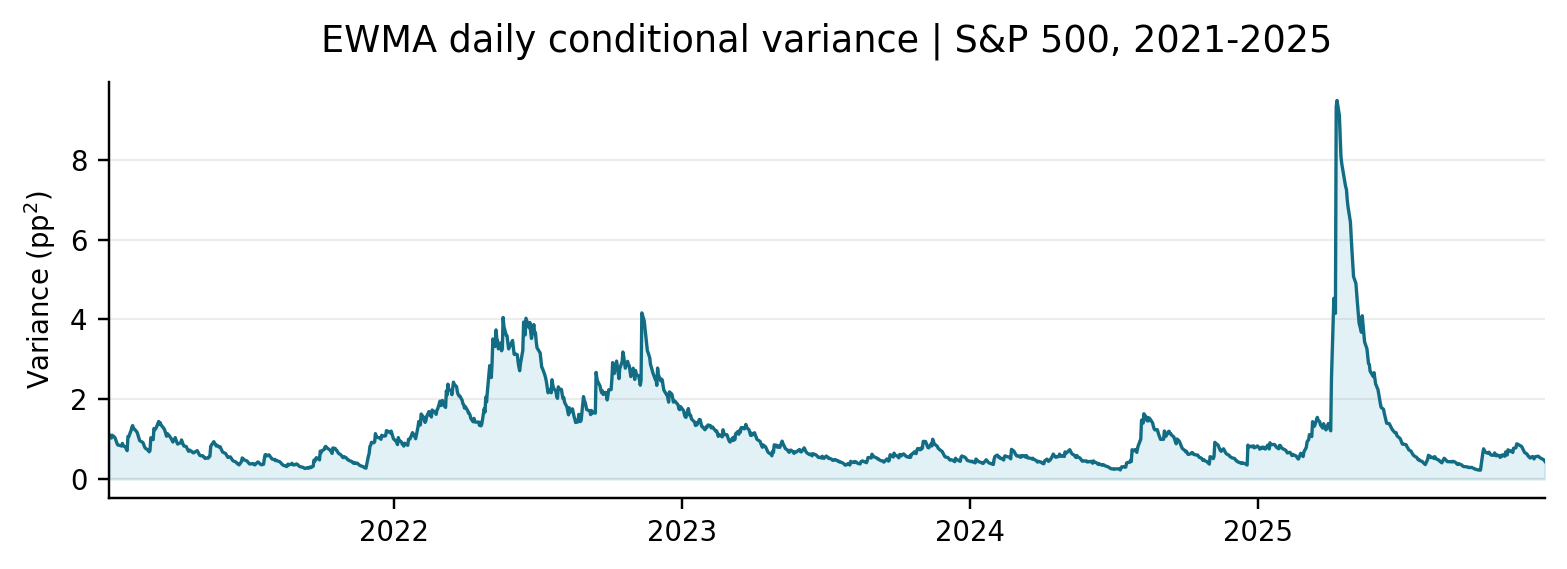
\includegraphics[width=0.98\linewidth]{figure_1_ewma_variance.png}
\caption{Daily EWMA forecast variance $\sigma_t^2$ from 2021 to 2025; replicated as an editable native Excel chart.}
\end{figure}

\newpage
\parthead{(b) Normal distribution: 5\% and 1\% daily VaR and backtesting}
For a long S\&P 500 position with conditional mean zero, define $\mathrm{VaR}_{\alpha,t}>0$ as the percentage \emph{loss magnitude} such that $P(R_t<-\mathrm{VaR}_{\alpha,t})=\alpha$. If $R_t\mid\mathcal{F}_{t-1}\sim N(0,\sigma_t^2)$, then
\begin{equation}
\boxed{\ \mathrm{VaR}^{N}_{\alpha,t}=-\Phi^{-1}(\alpha)\sigma_t\ },\quad
\begin{cases}
\mathrm{VaR}^{N}_{5\%,t}=1.644854\,\sigma_t,\\
\mathrm{VaR}^{N}_{1\%,t}=2.326348\,\sigma_t.
\end{cases}\label{eq:nvar}
\end{equation}
A VaR exception occurs on date $t$ if the \emph{realized} daily return $R_t<-\mathrm{VaR}_{\alpha,t}$. The target number of exceptions over $N=1255$ days is $N\alpha$: 62.75 for 5\%, and 12.55 for 1\%.

\begin{figure}[htbp]
\centering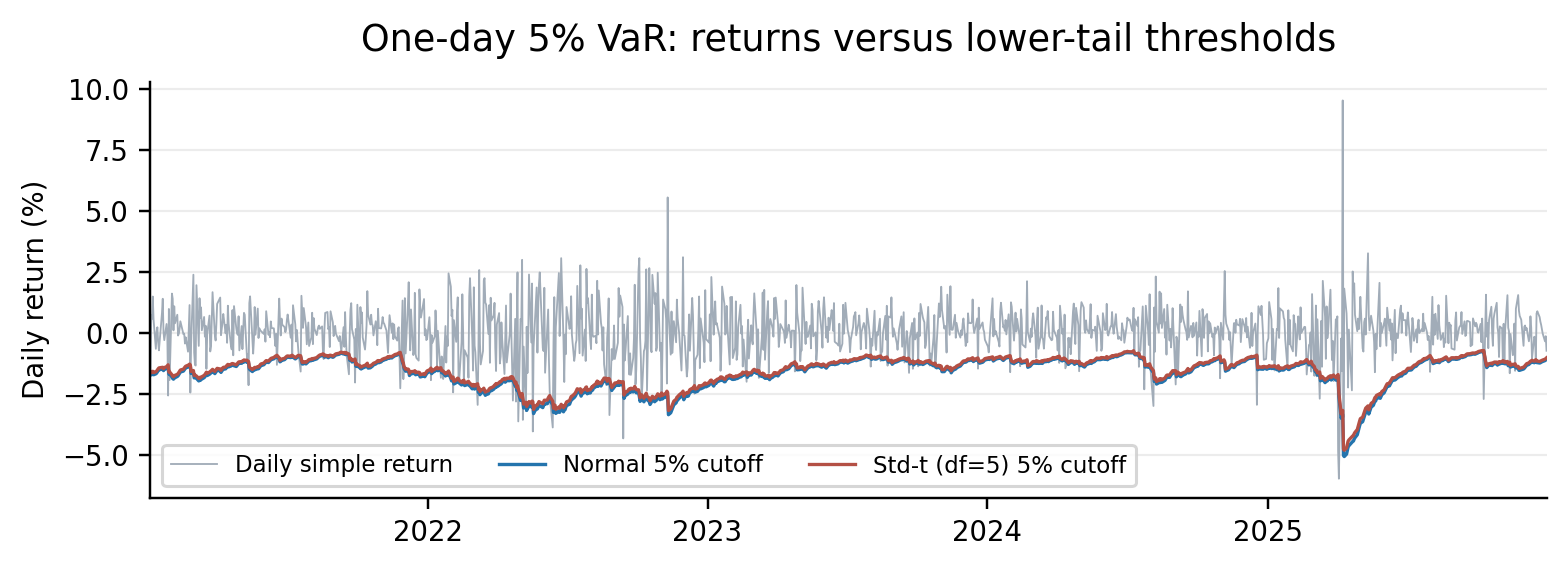
\includegraphics[width=0.98\linewidth]{figure_2_var_5pct.png}
\caption{Daily returns and negative 5\% VaR thresholds, normal and standardized-$t$ models. A breach occurs when the gray realized-return line is below the relevant threshold.}
\end{figure}

\begin{center}
\small
\begin{tabular}{@{}crrrrr@{}}\toprule
& & \multicolumn{2}{c}{Normal model exceptions} & \multicolumn{2}{c}{Standardized-$t$ exceptions} \\
\cmidrule(lr){3-4}\cmidrule(l){5-6}
Year & Days & 5\% & 1\% & 5\% & 1\% \\
\midrule
2021 & 252 & 12 & 8 & 12 & 7 \\
2022 & 251 & 20 & 4 & 22 & 2 \\
2023 & 250 & 13 & 2 & 15 & 0 \\
2024 & 252 & 14 & 6 & 16 & 5 \\
2025 & 250 & 15 & 6 & 16 & 5 \\
\midrule
\textbf{Total} & \textbf{1255} & \textbf{74} & \textbf{26} & \textbf{81} & \textbf{19} \\
\bottomrule
\end{tabular}
\end{center}

\textbf{Performance criterion.} To assess coverage, let $K$ denote the total number of exceptions and $\hat p=K/N$. Under the null hypothesis $H_0:p=\alpha$, the Kupiec unconditional-coverage likelihood-ratio statistic is
\begin{equation}
LR_{\mathrm{UC}}=2\left[K\ln\left(\frac{\hat p}{\alpha}\right)+(N-K)\ln\left(\frac{1-\hat p}{1-\alpha}\right)\right]
\ \overset{H_0}{\approx}\ \chi_1^2.\label{eq:kupiec}
\end{equation}
For the \textbf{normal 5\% VaR}, the observed rate is $74/1255=5.90\%$, $LR_{\mathrm{UC}}=2.013$, and $p=0.156$: \emph{do not reject} correct coverage at the 5\% significance level. For the \textbf{normal 1\% VaR}, the observed rate is $26/1255=2.07\%$, $LR_{\mathrm{UC}}=11.122$, and $p=0.00085$: \emph{reject} correct coverage; this VaR substantially underestimates extreme downside risk.

\newpage
\parthead{(c) Standardized Student's $t$ density and percentiles}
Let $X\sim t_\nu$ be an ordinary Student's $t$ random variable with $\nu>2$ degrees of freedom and density
\[
f_X(x)=\frac{\Gamma((\nu+1)/2)}{\sqrt{\nu\pi}\,\Gamma(\nu/2)}\left(1+\frac{x^2}{\nu}\right)^{-(\nu+1)/2},\qquad x\in\mathbb{R}.
\]
Define $Y=cX$ where $c=\sqrt{(\nu-2)/\nu}$. Because $x=y/c$ and $dx/dy=1/c$, the change-of-variables formula gives
\begin{align*}
f_Y(y)&=\frac{1}{c}f_X\!\left(\frac{y}{c}\right)\\
&=\boxed{\ \frac{\Gamma((\nu+1)/2)}{\sqrt{(\nu-2)\pi}\,\Gamma(\nu/2)}
\left(1+\frac{y^2}{\nu-2}\right)^{-(\nu+1)/2}\ },\qquad -\infty<y<\infty.
\end{align*}
As $\operatorname{Var}(X)=\nu/(\nu-2)$, it follows that $E(Y)=0$ and $\operatorname{Var}(Y)=1$. Let $t_\nu^{-1}(\alpha)$ denote the $\alpha$-quantile of the ordinary $t_\nu$ distribution. Since $c>0$, the required percentiles of the \emph{standardized} $t$ distribution are
\begin{equation}
\boxed{\ q_{0.01}(Y)=\sqrt{\frac{\nu-2}{\nu}}\,t_\nu^{-1}(0.01),\qquad
q_{0.05}(Y)=\sqrt{\frac{\nu-2}{\nu}}\,t_\nu^{-1}(0.05)\ }.\label{eq:tquant}
\end{equation}
The expressions above hold for any $\nu>2$. For the numerical example $\nu=5$,
\[
q_{0.01}(Y)=\boxed{-2.606464},\qquad q_{0.05}(Y)=\boxed{-1.560850}.
\]

\parthead{(d) Standardized-$t$ RiskMetrics VaR and comparison}
Suppose $R_t=\sigma_tY_t$ conditionally, with $Y_t$ distributed as the standardized Student's $t$ in part (c). Using the \emph{same} EWMA $\sigma_t$ from (a),
\begin{equation}
\boxed{\ \mathrm{VaR}^{t}_{\alpha,t}=-\sigma_t\sqrt{\frac{\nu-2}{\nu}}\,t_\nu^{-1}(\alpha)\ },\quad
\begin{cases}
\mathrm{VaR}^{t}_{5\%,t}=1.560850\,\sigma_t,\\
\mathrm{VaR}^{t}_{1\%,t}=2.606464\,\sigma_t
\end{cases}\ (\nu=5).
\end{equation}

\begin{figure}[htbp]
\centering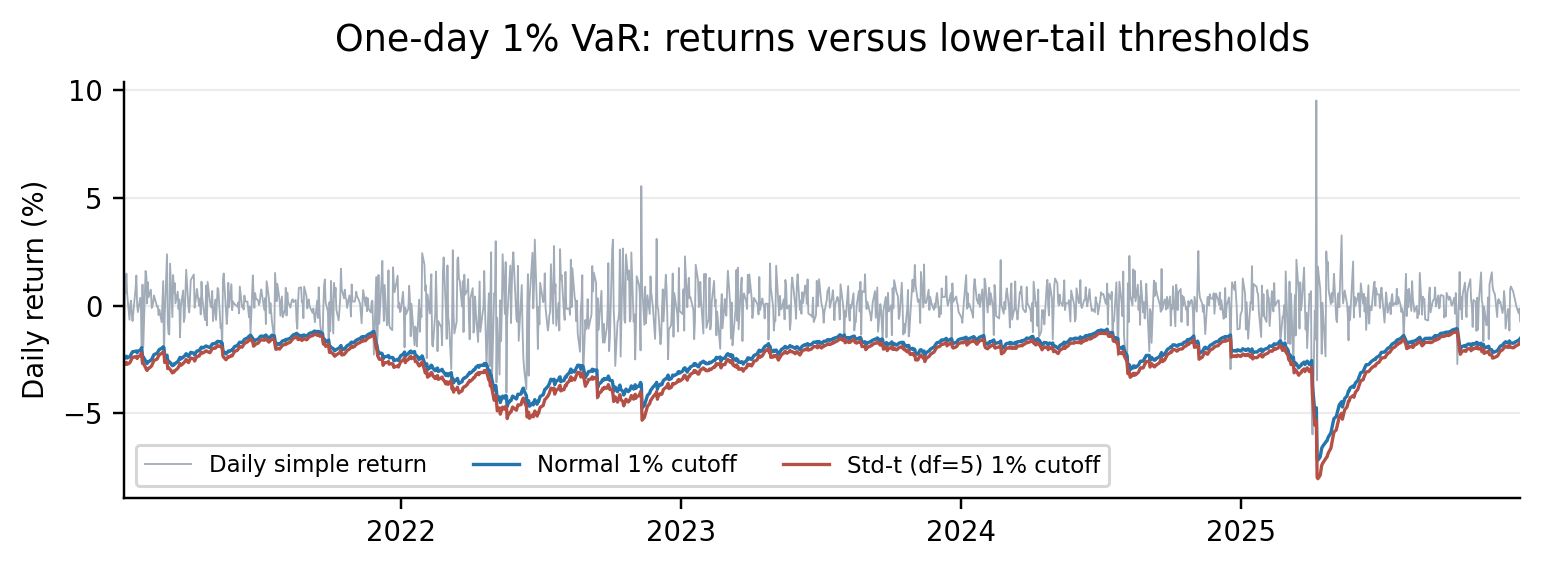
\includegraphics[width=0.98\linewidth]{figure_3_var_1pct.png}
\caption{Daily returns and negative 1\% VaR thresholds. With $\nu=5$, the standardized-$t$ model sets a more conservative 1\% threshold than the normal model.}
\end{figure}

\newpage
\parthead{VaR comparison and assessment (continuation of part d)}
Applying exactly the same exception rule and likelihood-ratio test to all four VaR series gives the following \emph{out-of-sample daily forecasts within the specified window}, subject to the fixed model parameters stated on page 1:

\begin{center}
\small
\begin{tabular}{@{}lrrrrl@{}}\toprule
Method & Tail & Expected & Observed & Rate & Kupiec $p$-value \\
\midrule
Normal & 5\% & 62.75 & 74 & 5.90\% & 0.1560 \\
Normal & 1\% & 12.55 & 26 & 2.07\% & 0.0009 \\
Standardized $t_5$ & 5\% & 62.75 & 81 & 6.45\% & 0.0234 \\
Standardized $t_5$ & 1\% & 12.55 & 19 & 1.51\% & 0.0890 \\
\bottomrule
\end{tabular}
\end{center}

\textbf{Interpretation of the 5\% and 1\% confidence assessments.}
\begin{itemize}[leftmargin=1.6em,itemsep=3pt,topsep=3pt]
\item \textbf{5\% VaR:} the normal model's observed 5.90\% breach frequency is closer to the nominal 5\% than the standardized-$t_5$ model's 6.45\%. The normal model passes the 5\%-significance Kupiec test ($p=0.156$), whereas the standardized-$t_5$ model fails ($p=0.0234$).
\item \textbf{1\% VaR:} the standardized-$t_5$ model reduces breaches from 26 to 19 and increases the loss quantile coefficient from 2.326348 to 2.606464. It passes the 5\%-significance Kupiec test ($p=0.089$), while the normal model fails ($p<0.001$). However, its realized breach rate of 1.51\% still exceeds the nominal 1\%, so the improvement is incomplete.
\item \textbf{Why this pattern occurs:} after variance standardization, Student's $t$ with $\nu=5$ has a \emph{smaller} 5\% loss coefficient but a \emph{larger} 1\% loss coefficient than the Gaussian model. Heavy tails mainly change the more extreme quantiles. A larger daily positive return also raises the next day's volatility forecast because the RiskMetrics update uses squared returns.
\item \textbf{Limitations:} unconditional exception frequency alone does not prove that exceptions are independent. A complete risk-model evaluation should additionally consider exception clustering (conditional coverage), model-parameter sensitivity, and economic loss from large breaches. The chosen $\nu=5$ is an explicit illustration, not an estimated or instructor-given parameter.
\end{itemize}

\textbf{Final conclusion.}
For the 2021--2025 S\&P 500 sample and the stated assumptions, \emph{normal EWMA VaR is better calibrated at the 5\% level, while standardized-$t_5$ EWMA VaR is better calibrated at the 1\% level}. Neither specification should be described as uniformly best at both confidence levels.

\vspace{7pt}\textbf{Data sources and clickable companion references.}
\begin{enumerate}[leftmargin=1.8em,itemsep=2pt,topsep=2pt]
\item S\&P Dow Jones Indices LLC, \emph{S\&P 500 [SP500]}, Federal Reserve Bank of St. Louis (FRED): \href{https://fred.stlouisfed.org/series/SP500}{\textcolor{blue!55!black}{official series}} and \href{https://fred.stlouisfed.org/data/SP500}{\textcolor{blue!55!black}{daily source table}}.
\item Historical price mirror: \href{https://github.com/AguilarMike/marketobservatory/blob/main/data/sp500.csv}{\textcolor{blue!55!black}{FRED price CSV mirror}}. Final 2025 observations were checked against FRED.
\item Reproducible project files: \href{https://github.com/YongWilliam-ai/ISOM3540_ass3_2026/blob/main/analysis.csv}{\textcolor{blue!55!black}{daily VaR calculations (CSV)}}, \href{https://github.com/YongWilliam-ai/ISOM3540_ass3_2026/blob/main/all_closes.csv}{\textcolor{blue!55!black}{S\&P 500 closing prices (CSV)}}, \href{https://github.com/YongWilliam-ai/ISOM3540_ass3_2026/blob/main/ISOM3540_21089310_ass3.tex}{\textcolor{blue!55!black}{LaTeX source}}, and \href{https://github.com/YongWilliam-ai/ISOM3540_ass3_2026/blob/main/README.md}{\textcolor{blue!55!black}{repository documentation}}.
\item The separately supplied editable \texttt{ISOM3540\_21089310\_ass3\_Excel.xlsx} has the \texttt{Assumptions}, \texttt{Warmup\_2020}, \texttt{Daily\_Data}, \texttt{Backtest} and \texttt{Excel\_Charts} sheets. Its GitHub publication status is recorded in the README.
\end{enumerate}
\end{document}